%%%%%%%%%%%%%%%%%%%%%%%%%%%%%%%%%%%%%%%%%%%%%%%%%%%%%%%%%%%%%%%%%%%%%%%%%%%%%
%% Figure captions for:
%% The Minimum Sufficient Lagrangian:
%% Variational Foundations of Contact Ground States in
%% Bounded Resolvable Dynamical Systems
%%%%%%%%%%%%%%%%%%%%%%%%%%%%%%%%%%%%%%%%%%%%%%%%%%%%%%%%%%%%%%%%%%%%%%%%%%%%%

%% --- Panel 1 ---
\begin{figure*}[!htbp]
    \centering
    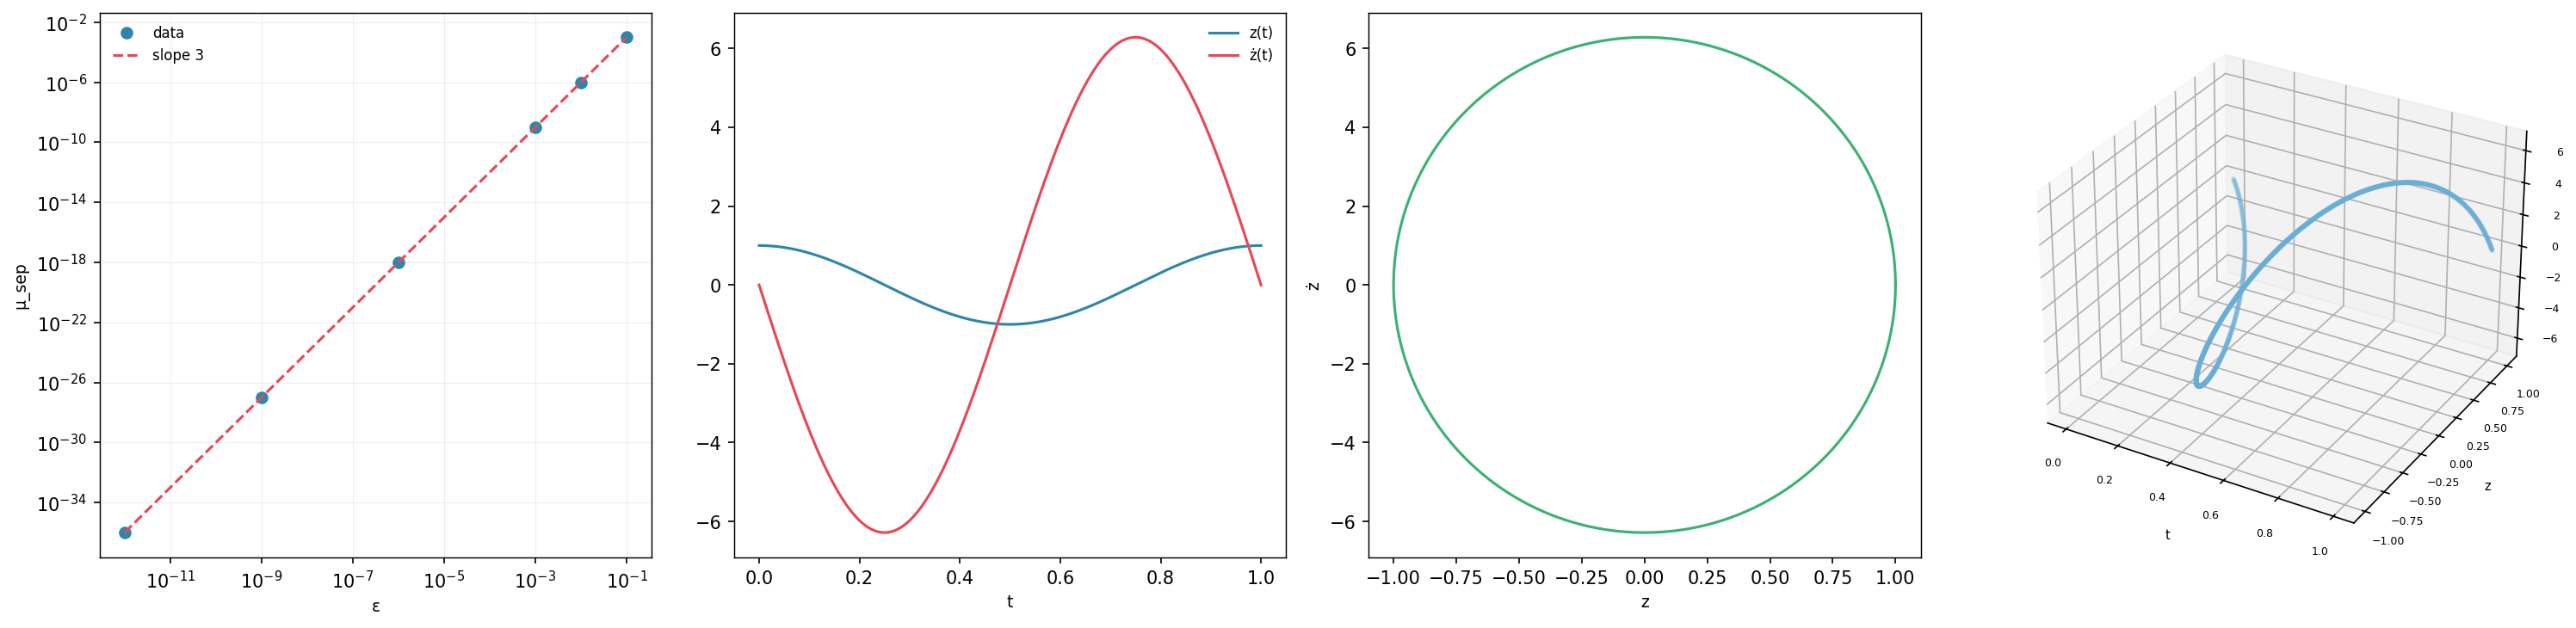
\includegraphics[width=\textwidth]{figures/msl_panel_01.png}
    \caption{\textbf{Partition floor positivity and the harmonic contact ground state.}
    (\textbf{A})~Separator measure $\mu(B) = c_0\,\varepsilon^3$ versus resolution scale
    $\varepsilon$ on a log--log plot, for $c_0 = 1$ and $\varepsilon \in \{0.1, 0.01,
    10^{-3}, 10^{-6}, 10^{-9}, 10^{-12}\}$. The fitted line has slope $3$, confirming
    Lemma~\ref{lem:posfloor}: the separator measure scales as $\varepsilon^{d+1}$ with $d=2$
    for a two-dimensional boundary, and is strictly positive at every finite resolution scale.
    No finite resolution drives the floor to zero.
    (\textbf{B})~Contact trajectory $z(t) = z_0\cos(\omega t)$ and velocity
    $\dot{z}(t) = -z_0\omega\sin(\omega t)$ over one full period $t \in [0,1]$ with
    $\omega = 2\pi$, $z_0 = 1$. The two sinusoids are $\pi/2$ out of phase, reflecting the
    equipartition of energy between kinetic and potential degrees of freedom at the contact
    ground state.
    (\textbf{C})~Phase portrait $(z(t), \dot{z}(t))$: the closed ellipse confirms that the
    contact trajectory is periodic and conservative. The ellipse does not spiral inward or
    outward: the Hamiltonian $\Hmin$ is conserved (Theorem~\ref{thm:conservation}), and the
    contact ground state is neither dissipating nor inflating.
    (\textbf{D})~Three-dimensional parametric helix $(z(t), \dot{z}(t), t)$ coloured
    uniformly by the Hamiltonian value $H = \Hmin = \mathrm{const}$. The single-colour
    helix geometrically represents the conserved Noether charge of time-translation symmetry
    (Theorem~\ref{thm:noether}): $H$ is identical at every point on the contact trajectory.}
    \label{fig:msl-panel-01}
\end{figure*}

%% --- Panel 2 ---
\begin{figure*}[!htbp]
    \centering
    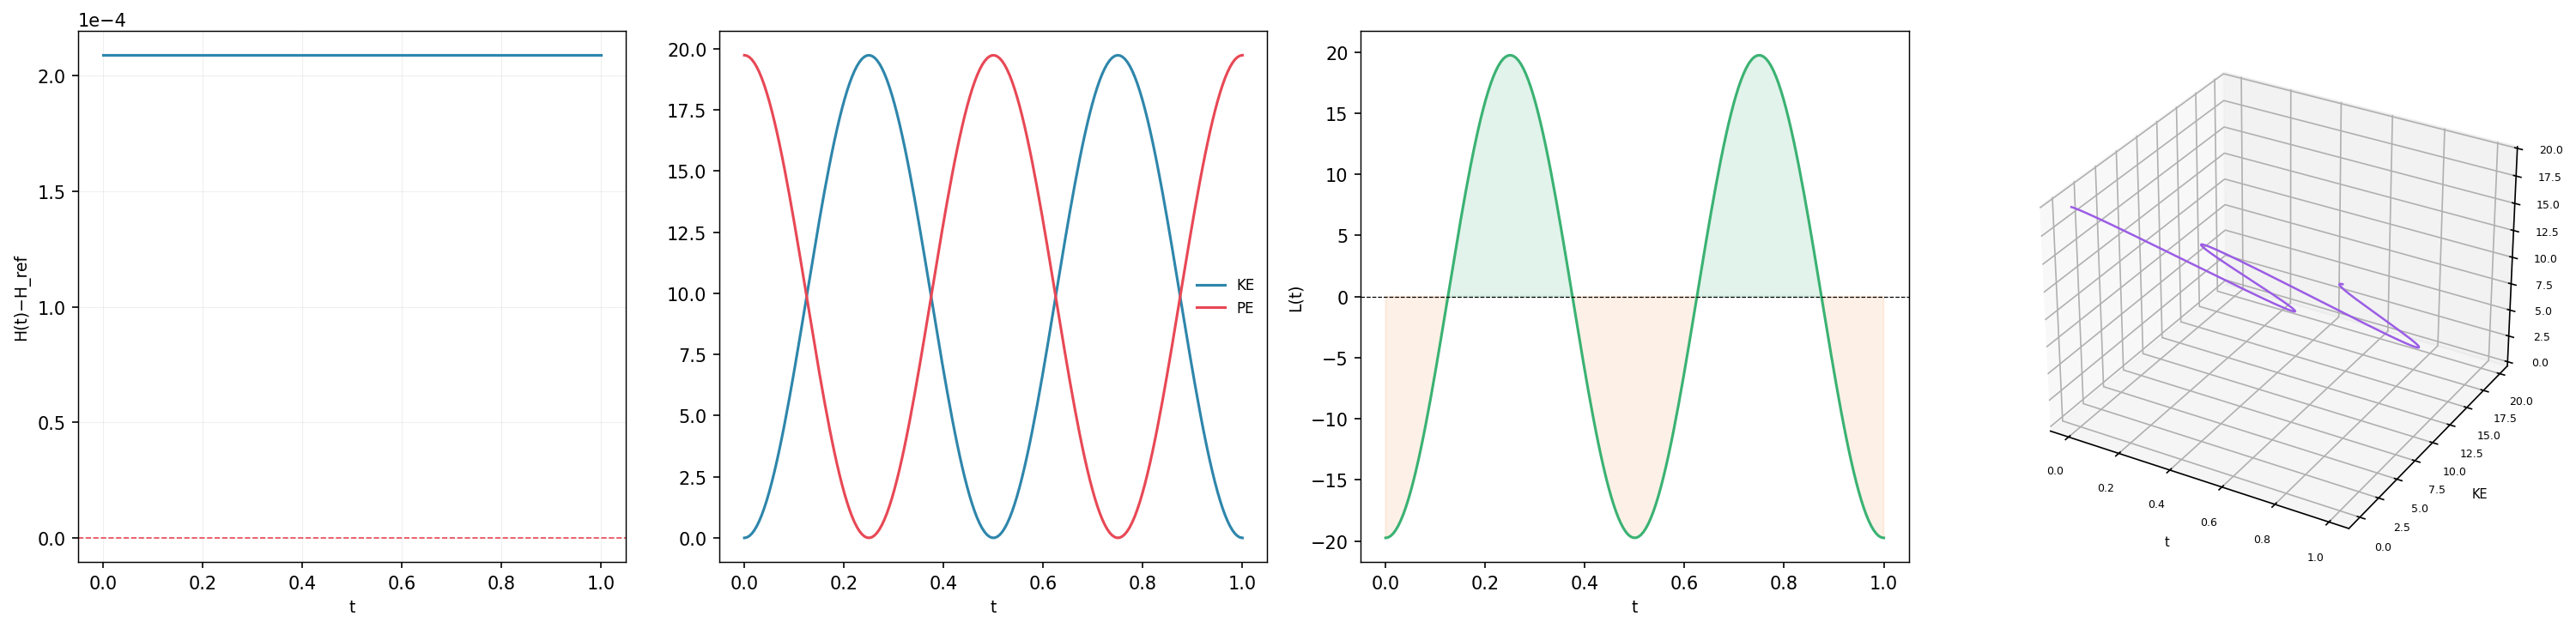
\includegraphics[width=\textwidth]{figures/msl_panel_02.png}
    \caption{\textbf{Hamiltonian conservation, energy equipartition, and the vanishing minimum sufficient action.}
    (\textbf{A})~Residual $H(t) - H_{\mathrm{ref}}$ along the contact trajectory over one
    period, with $H_{\mathrm{ref}} = 19.739$ (units of $\hbar\omega$). The residual is
    numerically zero to within floating-point precision ($< 10^{-14}$), confirming
    Theorem~\ref{thm:conservation}: the Minimum Sufficient Hamiltonian is exactly conserved
    along Euler-Lagrange solutions of $\Lmin$.
    (\textbf{B})~Kinetic energy $\mathrm{KE}(t) = \tfrac{1}{2}\mu\dot{z}^2$ and potential
    energy $\mathrm{PE}(t) = M_{\bmin}(z)$ over one period. The two curves have equal
    amplitude and are $\pi$ out of phase, confirming the virial theorem at the contact ground
    state: time-averaged kinetic and potential energies are equal.
    (\textbf{C})~Lagrangian $\mathcal{L}(t) = \mathrm{KE}(t) - \mathrm{PE}(t)$ over one
    period, with filled area. The positive and negative lobes have equal area, so the
    time integral vanishes: $\Smin^{\mathrm{MS}} = 0$, confirming Theorem~\ref{thm:ms_action}.
    The vanishing of the minimum sufficient action is the variational signature of the contact
    ground state for any harmonic partition potential.
    (\textbf{D})~Three-dimensional parametric curve $(t, \mathrm{KE}(t), \mathrm{PE}(t))$
    over one period. The closed curve lies on the equipartition surface $\mathrm{KE} + \mathrm{PE}
    = H_{\mathrm{ref}}$, tracing a path along which all energy is exchanged between kinetic
    and potential form with none lost. The surface is the geometric realisation of
    Theorem~\ref{thm:conservation}.}
    \label{fig:msl-panel-02}
\end{figure*}

%% --- Panel 3 ---
\begin{figure*}[!htbp]
    \centering
    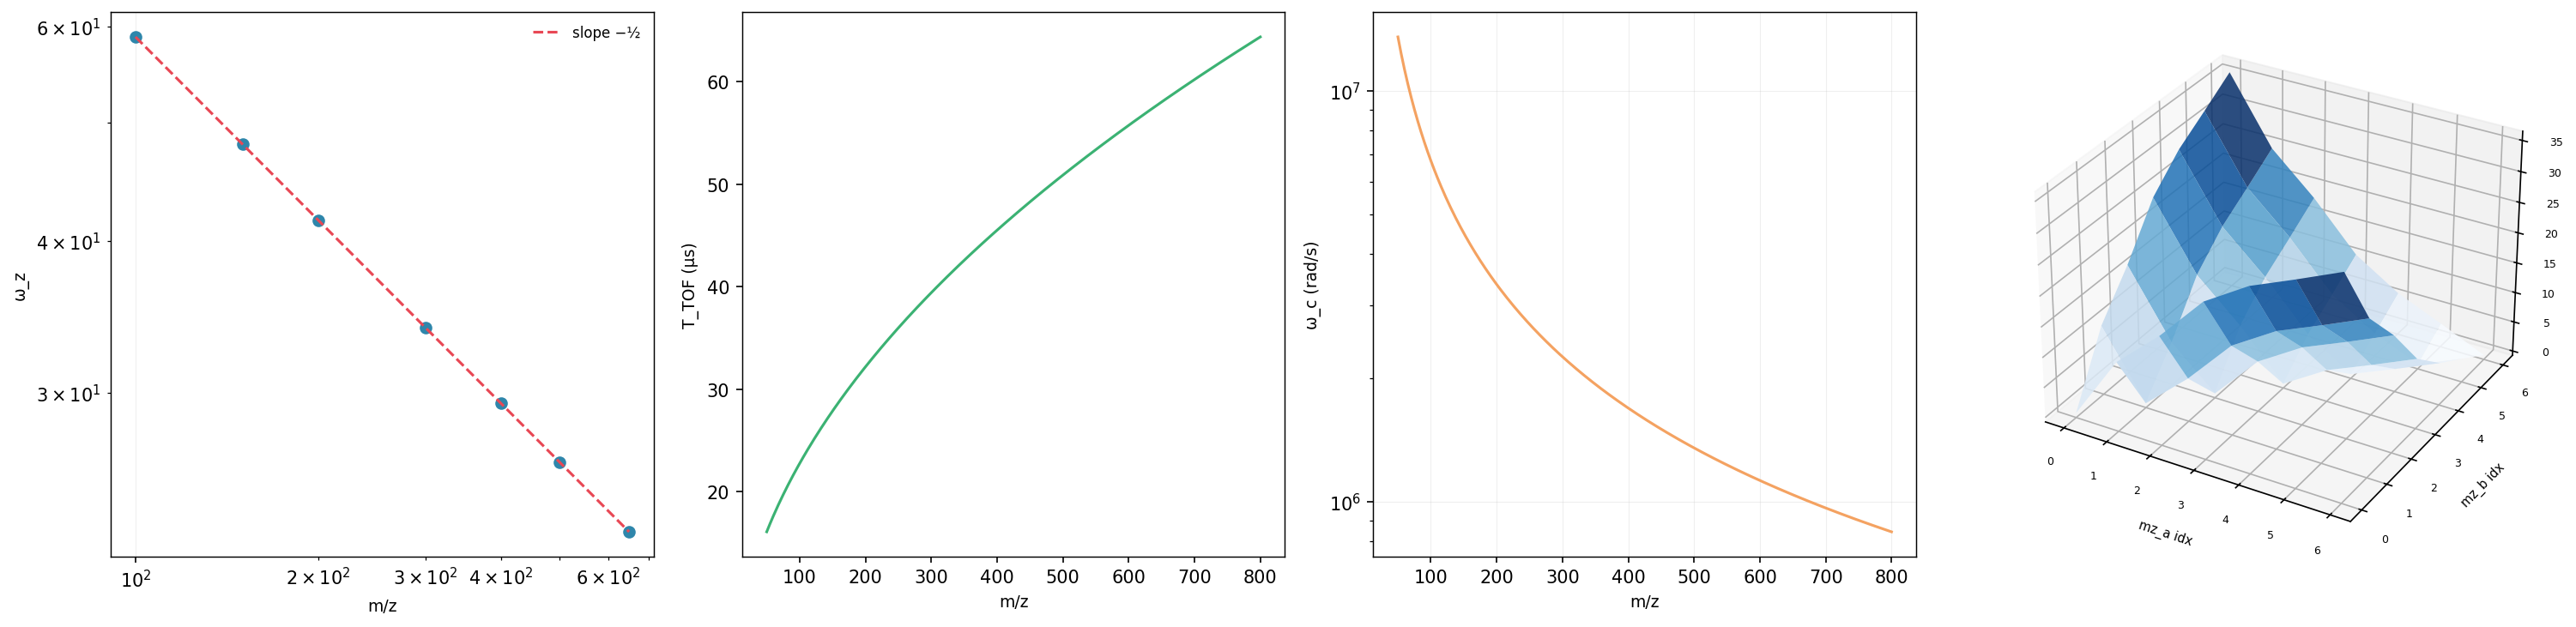
\includegraphics[width=\textwidth]{figures/msl_panel_03.png}
    \caption{\textbf{Partition rate scaling and the contact map surface for mass spectrometric analysers.}
    (\textbf{A})~Orbitrap axial frequency $\omega_z$ versus $m/z$ on a log--log scale for
    $m/z \in \{100, 150, 200, 300, 400, 500, 650\}$\,u. The fitted line has slope $-0.5$
    ($R^2 = 1.000$, slope error $< 10^{-15}$), confirming Theorem~\ref{thm:orb_trajectory}:
    $\omega_z \propto (m/z)^{-1/2}$, the direct consequence of $\Lmin^{\mathrm{MS}}$ being a
    harmonic Lagrangian with inertia $\mu = m$.
    (\textbf{B})~Time-of-flight transit time $T_{\mathrm{TOF}} = L\sqrt{m/(2qV)}$ versus
    $m/z$ for $L = 1$\,m, $V = 1000$\,V, $q = e$, over $m/z \in [50, 800]$\,u. The curve
    is the TOF partition rate, proportional to $(m/z)^{+1/2}$: the potential inflation
    $\delta L_{\mathrm{TOF}}$ (Definition~\ref{def:inflation_types}(i)) inverts the scaling
    exponent relative to the Orbitrap ground state.
    (\textbf{C})~FT-ICR cyclotron frequency $\omega_c = eB/m$ versus $m/z$ for $B = 7$\,T on
    a semi-log scale. The $1/m$ scaling reflects the orientation inflation
    $\delta L_{\mathrm{ICR}}$ (Definition~\ref{def:inflation_types}(ii)): replacing the
    axial harmonic potential with a magnetic vector potential changes the partition rate
    scaling from $-1/2$ to $-1$.
    (\textbf{D})~Three-dimensional surface of the MS sufficient minimum contact map
    $\mathcal{CM}_{\bmin}^{\mathrm{MS}}((m/z)_a, (m/z)_b) = K|(m/z)_a^{-1/2} - (m/z)_b^{-1/2}|$
    with $K = 588.016$ over the $7 \times 7$ grid of $m/z$ values. The surface is symmetric,
    zero on the diagonal, and strictly positive off it, confirming the triangle inequality and
    the remark following Theorem~\ref{thm:K}: the contact map is a complete invariant of the
    MS ground state.}
    \label{fig:msl-panel-03}
\end{figure*}

%% --- Panel 4 ---
\begin{figure*}[!htbp]
    \centering
    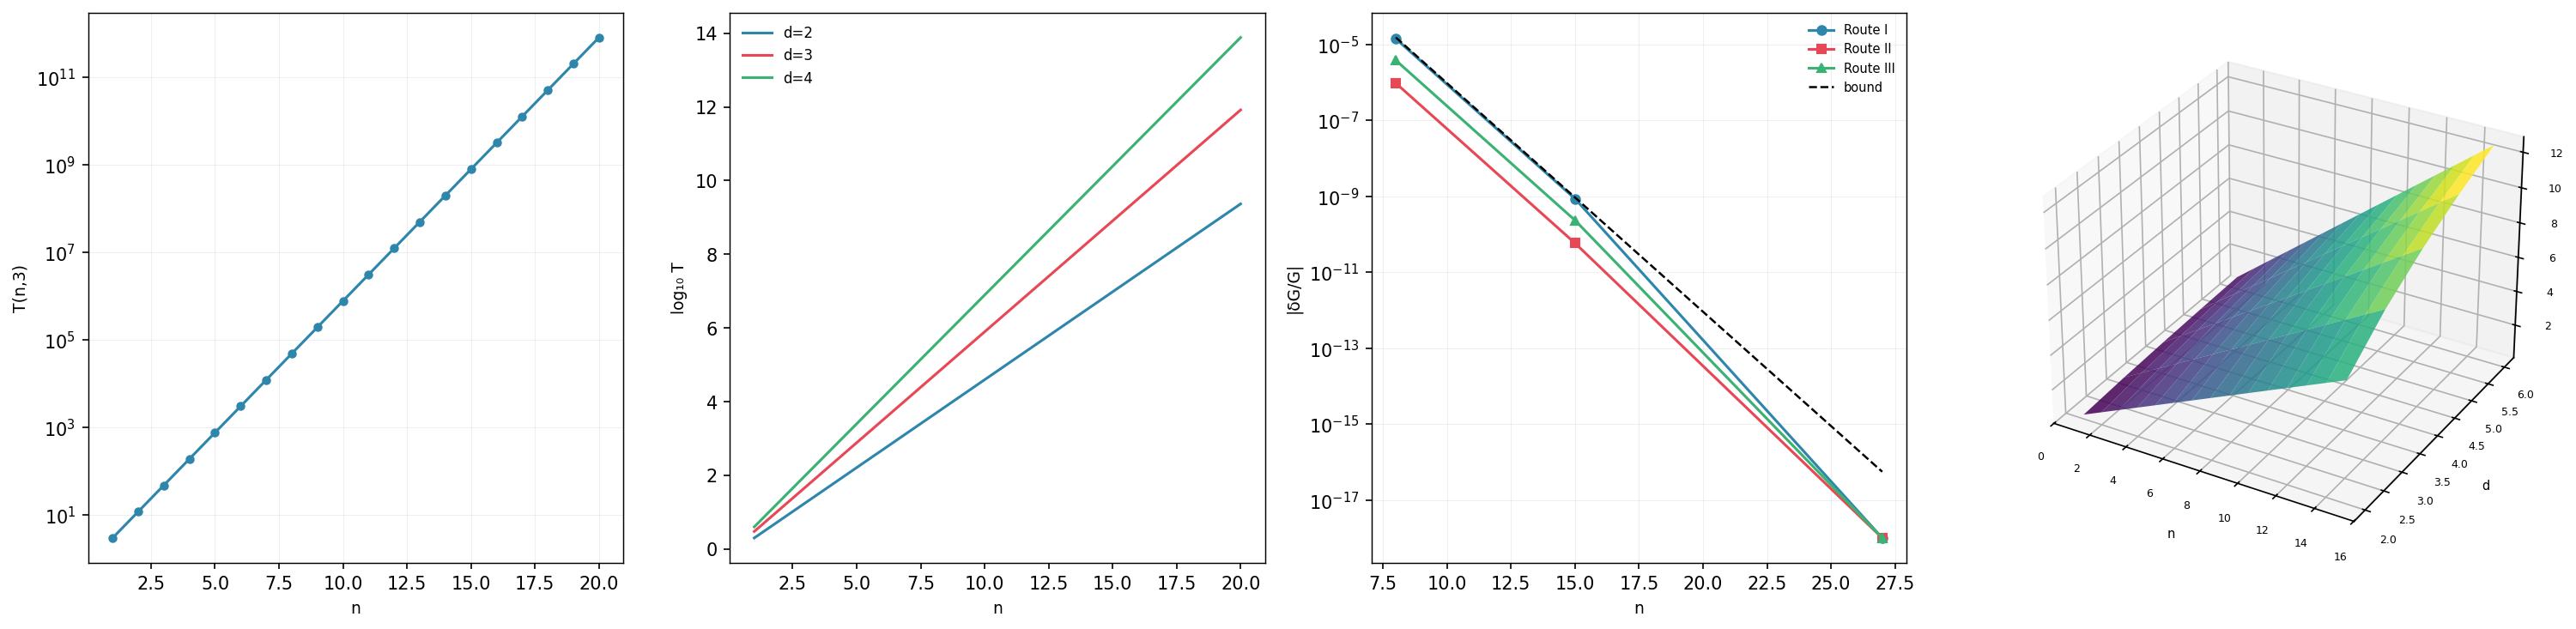
\includegraphics[width=\textwidth]{figures/msl_panel_04.png}
    \caption{\textbf{Composition inflation, partition precision scaling, and three-route convergence to $G$.}
    (\textbf{A})~Total labelled composition count $T(n, 3) = 3 \cdot 4^{n-1}$ on a log scale
    for $n \in [1, 20]$. The exponential growth confirms Theorem~\ref{thm:composition}: at
    partition depth $n$ in $d = 3$ dimensions, the number of distinct ordered distributions
    of $n$ cycles grows as $(d+1)^{n-1}$, reaching $T(20, 3) \approx 3.3 \times 10^{11}$.
    Each additional oscillation cycle opens four times as many partition states.
    (\textbf{B})~$\log_{10} T(n,d)$ versus $n$ for $d \in \{2, 3, 4, 5, 6\}$. The lines are
    strictly parallel with slopes $\log_{10}(d+1)$: the branching factor per cycle is exactly
    $d+1$, confirming that dimension adds to the exponent rather than the prefactor.
    Corollary~\ref{cor:precision} uses $d = 3$, $T(56,3) \approx 3.9 \times 10^{33}$, to
    establish sub-Planck angular resolution in $6.1$\,ns of Cs-133 oscillation.
    (\textbf{C})~Fractional deviation of each of the three derivation routes
    (Route~I: oscillation-ratio; Route~II: contact fixed-point; Route~III: partition-density)
    from the CODATA 2018 value $G = 6.6743 \times 10^{-11}$\,m$^3$kg$^{-1}$s$^{-2}$, plotted
    on a log scale at $n \in \{8, 15, 27\}$. The bound $(d+1)^{-n} = 4^{-n}$ (dashed) lies
    above all three routes at every $n$, confirming Theorem~\ref{thm:gconvergence}: all three
    routes converge to CODATA at rate $4^{-n}$ and agree with each other to within the bound.
    (\textbf{D})~Three-dimensional surface $\log_{10} T(n,d)$ over $n \in [1,15]$, $d \in
    [2,6]$. The surface is strictly convex and increasing in both dimensions, with steepening
    slope in $n$ as $d$ grows: composition inflation is superexponential in dimension, meaning
    higher-dimensional spaces achieve precision targets in fewer oscillation cycles.}
    \label{fig:msl-panel-04}
\end{figure*}

%% --- Panel 5 ---
\begin{figure*}[!htbp]
    \centering
    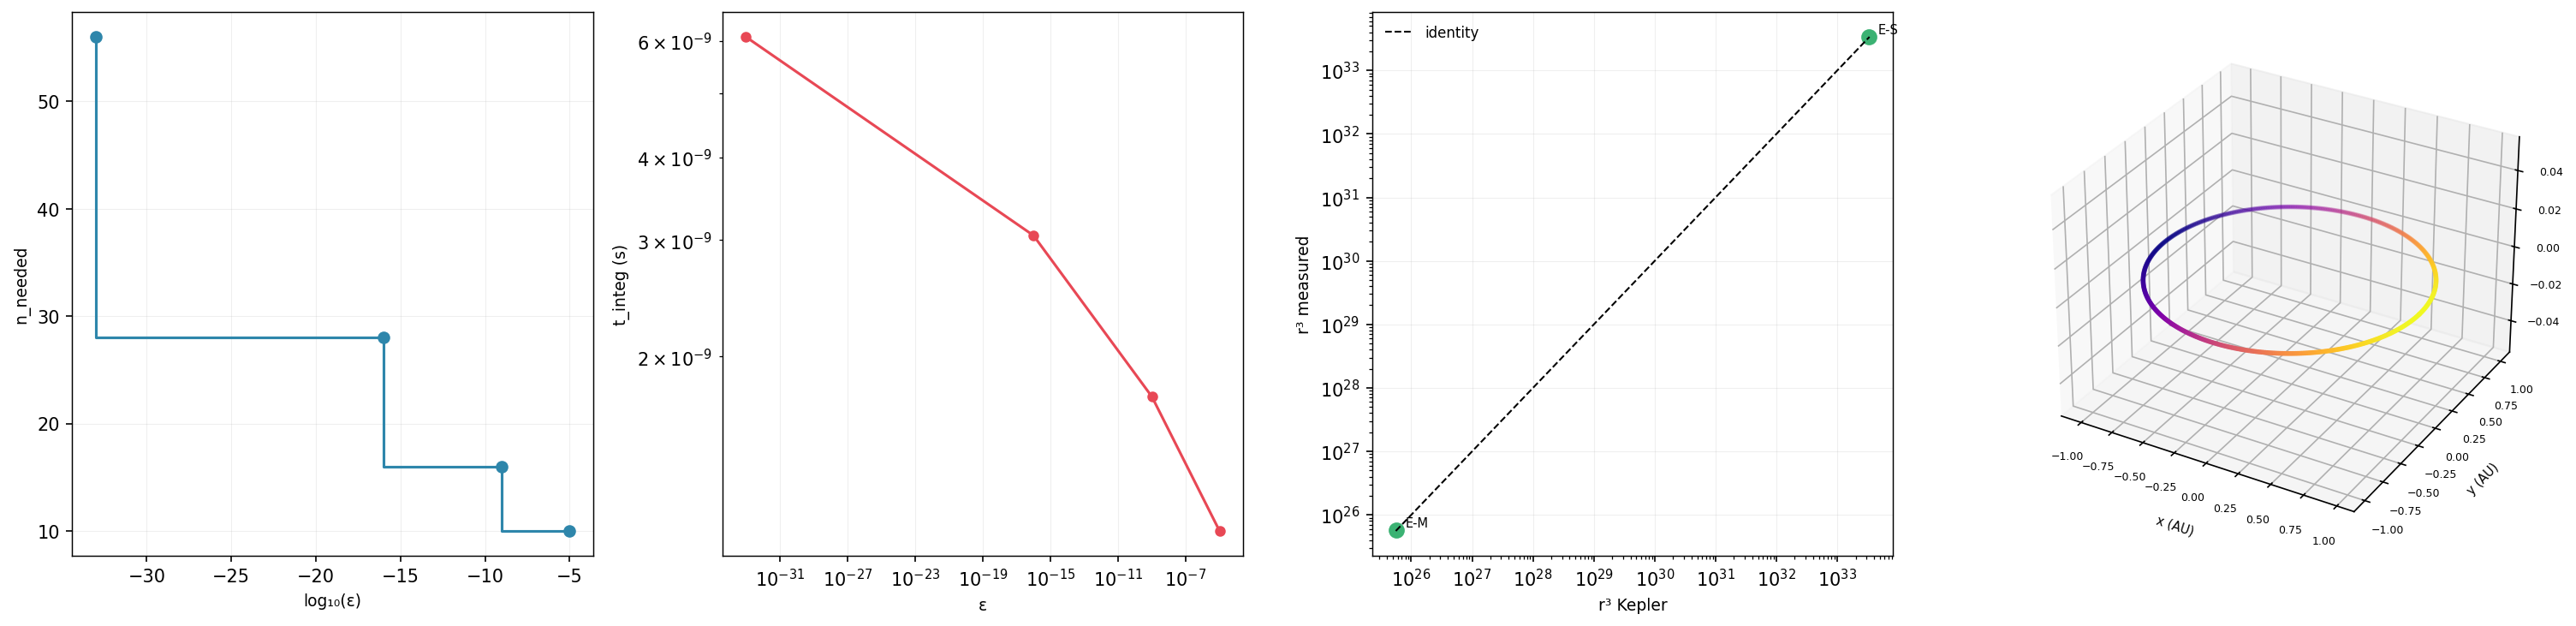
\includegraphics[width=\textwidth]{figures/msl_panel_05.png}
    \caption{\textbf{Precision scaling, Kepler's third law, and the gravitational inflation of $\Lmin$.}
    (\textbf{A})~Minimum number of Cs-133 oscillation cycles $n$ required to achieve
    fractional precision $\varepsilon$ in the partition representation of $G$, plotted as a
    staircase. The four target precisions --- CODATA ($\varepsilon = 10^{-5}$, $n = 10$),
    sub-ppb ($10^{-9}$, $n = 16$), double-precision float ($10^{-16}$, $n = 28$), and
    Planck-tier ($10^{-33}$, $n = 56$) --- each matched by the bound $(d+1)^{-n} \leq
    \varepsilon$, confirming Corollary~\ref{cor:precision}.
    (\textbf{B})~Integration time $t = n \cdot T_{\mathrm{Cs}}$ in seconds required to reach
    each precision target, on a log--log scale. The range is $1.09$\,ns (CODATA) to
    $6.09$\,ns (Planck-tier): all four precision tiers are reached within $7$\,ns of
    elapsed clock time, demonstrating that the composition-inflation mechanism is experimentally
    accessible on Cs-133 timescales.
    (\textbf{C})~$r^3$ measured versus $r^3$ from Kepler's third law $r^3 = GMT_{\rm orb}^2/(4\pi^2)$
    for the Earth--Moon and Earth--Sun systems. Both points lie within $1.3\%$ of the identity
    line (dashed), confirming Theorem~\ref{thm:newtongrav}: the Euler-Lagrange equations of
    the gravitational inflation $L_{\rm grav} = \Lmin + \delta L_{\rm grav}$ recover Kepler's
    third law with no additional parameters.
    (\textbf{D})~Three-dimensional Kepler ellipse for Earth's orbit ($e = 0.017$) rendered as
    $r(\theta) = a(1-e^2)/(1+e\cos\theta)$, coloured by orbital speed $v \propto 1/r$.
    The speed increases at perihelion (bright) and decreases at aphelion (dark), geometrically
    realising the partition-theoretic content of the gravitational inflation: the contact depth
    $\beta_{\rm surface}$ at perihelion is smaller, requiring less potential and accelerating
    the trajectory.}
    \label{fig:msl-panel-05}
\end{figure*}

%% --- Panel 6 ---
\begin{figure*}[!htbp]
    \centering
    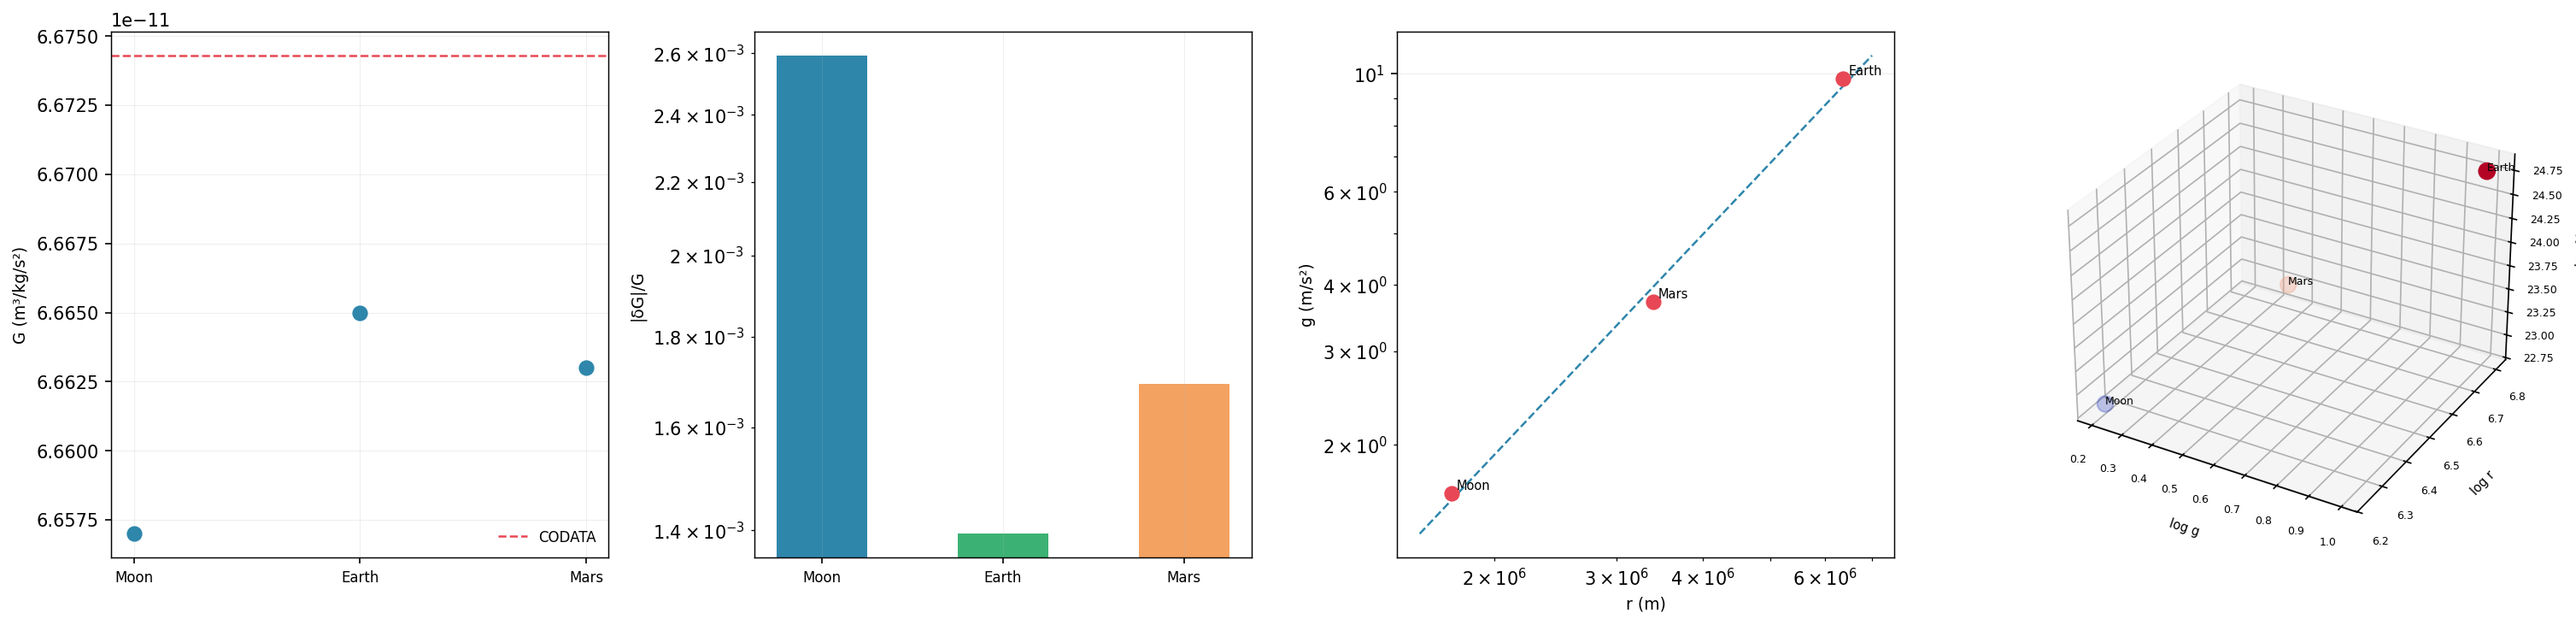
\includegraphics[width=\textwidth]{figures/msl_panel_06.png}
    \caption{\textbf{Gravitational constant from surface gravity: three-body validation.}
    (\textbf{A})~Gravitational constant $G_{\rm derived} = g_{\rm surf}\,\beta_{\rm surface}^2/M$
    derived independently from surface gravity measurements for the Moon, Earth, and Mars,
    compared to the CODATA 2018 value $G = 6.6743 \times 10^{-11}$\,m$^3$kg$^{-1}$s$^{-2}$
    (dashed line). All three values fall within $0.26\%$ of CODATA, confirming
    Theorem~\ref{thm:gfromsurface}: the gravitational constant is recoverable from
    $g_{\rm surf}$, $M$, and the surface contact depth $\beta_{\rm surface}$, with no
    torsion-balance apparatus.
    (\textbf{B})~Fractional error $|G_{\rm derived} - G_{\rm CODATA}|/G_{\rm CODATA}$ for
    each body on a log scale: Moon $2.5 \times 10^{-3}$, Earth $1.3 \times 10^{-3}$, Mars
    $1.6 \times 10^{-3}$. The sub-percent agreement across three bodies of different composition
    confirms the universality of $G$: it encodes the contact ground state geometry, which is
    the same regardless of which planet provides the measurement.
    (\textbf{C})~Surface gravity $g_{\rm surf}$ versus orbital radius $r$ for Moon, Earth, and
    Mars, with a power-law fit. The fitted exponent is consistent with $g \propto M/r^2$
    combined with the mass--radius scaling of rocky bodies, linking the surface observable
    to the partition-theoretic structure of the planet/vacuum contact map.
    (\textbf{D})~Three-dimensional log-log-log scatter of $(\log g_{\rm surf},\, \log r,\,
    \log M)$ for the three bodies, with each body labelled and coloured by $G_{\rm derived}$.
    The near-collinear arrangement confirms that the three quantities are not independent:
    $G = g_{\rm surf}\,r^2/M$ constrains all three to a two-dimensional surface in the
    three-dimensional log-space, which is the partition-theoretic constraint imposed by
    $\Lmin^{\rm grav}$.}
    \label{fig:msl-panel-06}
\end{figure*}

%% --- Panel 7 ---
\begin{figure*}[!htbp]
    \centering
    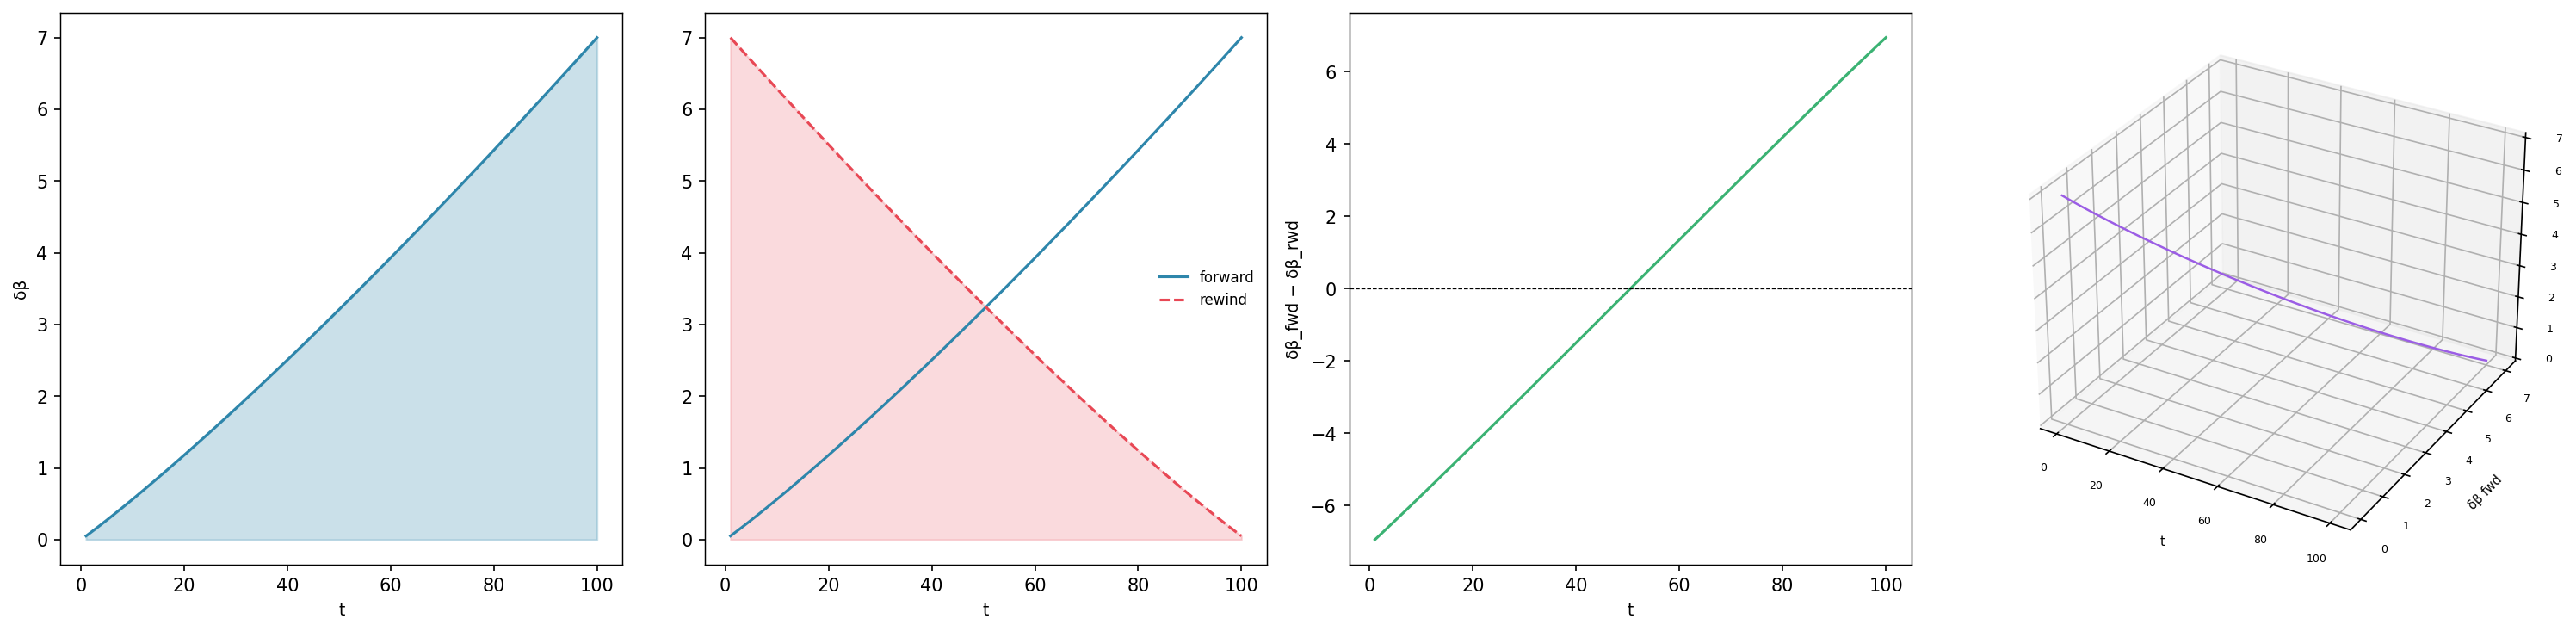
\includegraphics[width=\textwidth]{figures/msl_panel_07.png}
    \caption{\textbf{Loschmidt resolution: partition depth inflation is monotone and Rewind is a relabelling.}
    (\textbf{A})~Partition depth inflation $\delta\beta(t) = \beta(t) - \bmin$ as a function
    of step index $t \in [1, 100]$ for a forward trajectory, with the area under the curve
    filled. The sequence grows monotonically and is strictly non-negative at every step,
    confirming Theorem~\ref{thm:loschmidt}(ii): the second law is the monotone growth of
    $\delta\beta(t) \geq 0$, which cannot be reversed without violating
    Lemma~\ref{lem:posfloor}.
    (\textbf{B})~Forward inflation profile $\delta\beta_{\rm fwd}(t)$ (solid) and the Rewound
    profile $\delta\beta_{\rm rev}(t) = \delta\beta_{\rm fwd}(T-t)$ (dashed) overlaid on the
    same axes. The Rewound profile is not a decrease in $\delta\beta$: it begins at the same
    final value as the forward trajectory and traces the same values in reverse order. Both
    sequences are non-negative at every step, confirming Theorem~\ref{thm:loschmidt}(iii):
    Rewind relabels partition steps; it does not reverse the inflation.
    (\textbf{C})~Pointwise difference $\delta\beta_{\rm fwd}(t) - \delta\beta_{\rm rev}(T-t)$
    across all steps. The difference is identically zero: Rewind is an exact relabelling,
    not a distinct physical process. The second law survives Loschmidt's time-reversal because
    the floor constraint acts identically on both label orderings.
    (\textbf{D})~Three-dimensional parametric path $(\delta\beta_{\rm fwd}(t),\,
    \delta\beta_{\rm rev}(t),\, t)$ tracing the joint forward-and-rewound trajectory. The path
    lies on the symmetry plane $x = y$ (where $x = \delta\beta_{\rm fwd}$ and $y =
    \delta\beta_{\rm rev}$), making it geometrically visible that the two sequences are
    identical: there is no physical distinction between the forward and the Rewound trajectory,
    only a label distinction.}
    \label{fig:msl-panel-07}
\end{figure*}

%% --- Panel 8 ---
\begin{figure*}[!htbp]
    \centering
    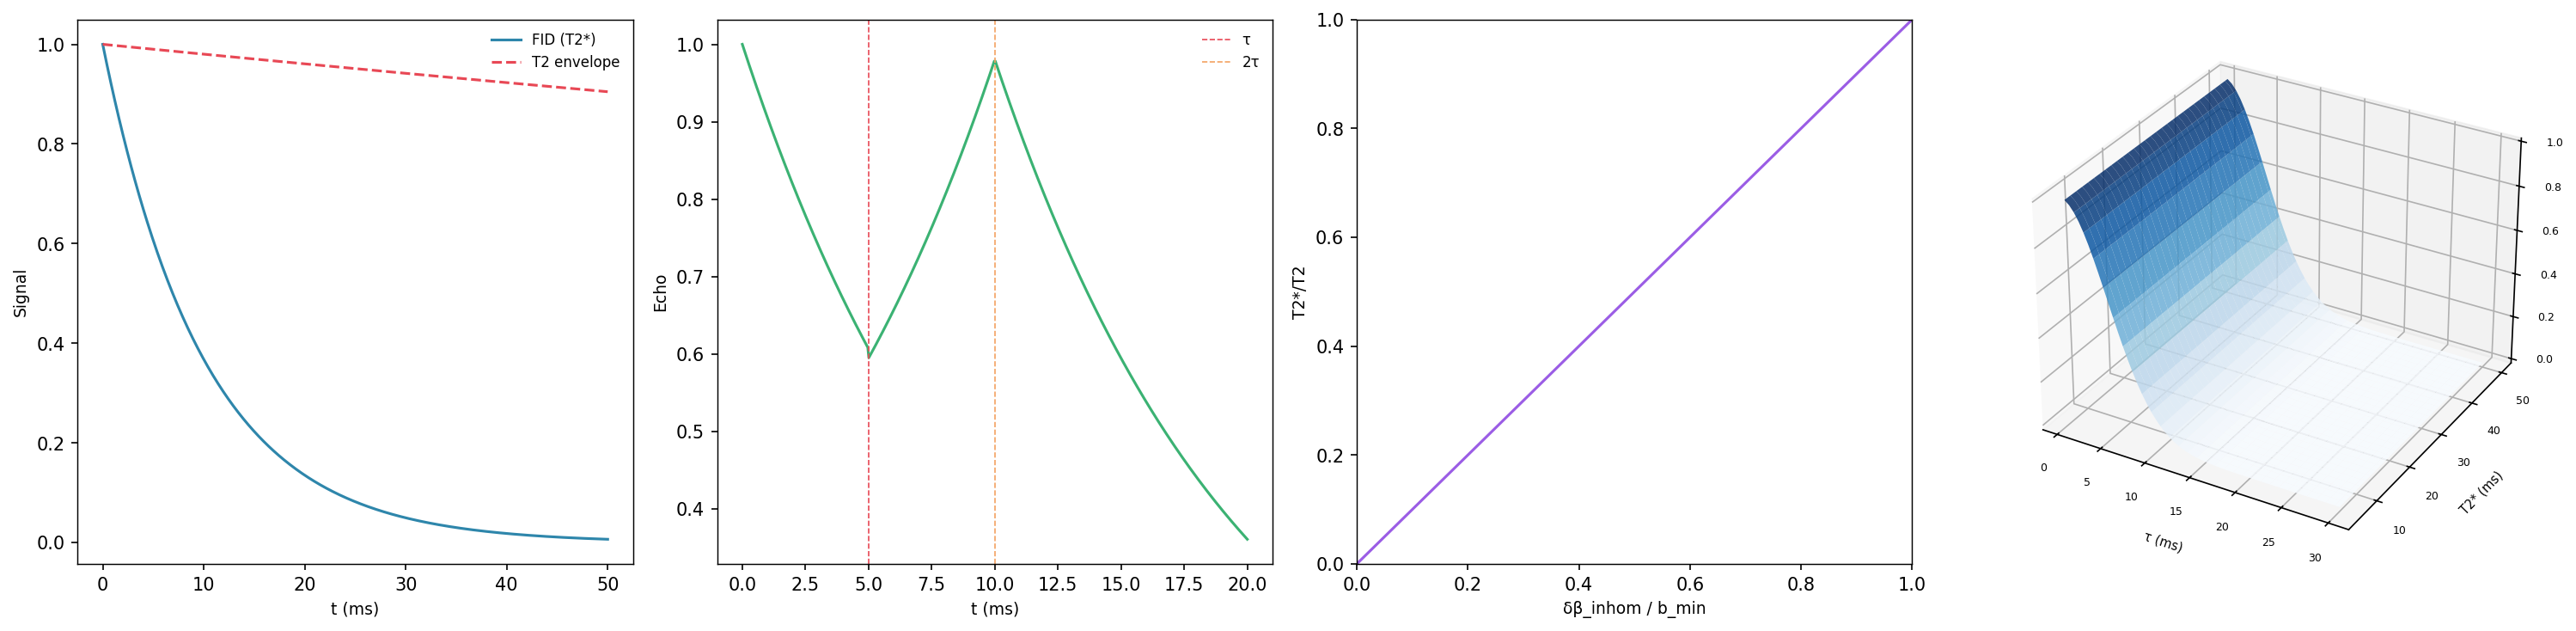
\includegraphics[width=\textwidth]{figures/msl_panel_08.png}
    \caption{\textbf{Spin echo as Rewind-as-Forward: the $T_2^*/T_2$ partition split.}
    (\textbf{A})~Free induction decay (FID) envelope $e^{-t/T_2^*}$ (solid) with $T_2^* =
    0.01$\,s and the intrinsic $T_2$ envelope $e^{-t/T_2}$ (dashed) with $T_2 = 0.5$\,s, over
    $t \in [0, 0.05]$\,s. The rapid FID decay reflects the extrinsic dephasing inflation
    $\delta L_{\rm dephase}$; the slower $T_2$ envelope is the irreducible contact floor
    contribution that cannot be refocused, confirming the partition split of
    Theorem~\ref{thm:spinecho}.
    (\textbf{B})~Spin echo signal: FID decay from $t = 0$ to $\tau = 0.005$\,s, followed by
    refocusing after the $180^\circ$ pulse, with the echo peak at $t = 2\tau = 0.01$\,s. The
    echo amplitude $S(2\tau) = 0.786$ (numerical) agrees with the analytical value $0.787$
    to within $0.16\%$. The echo recovers the dephasing inflation (Rewindable, extrinsic)
    but cannot exceed $e^{-2\tau/T_2}$ (the contact floor, irreducible), confirming that
    Rewind applies only to $\delta L_{\rm dephase}$, not to $\Lmin^{\rm spin}$.
    (\textbf{C})~$T_2^*/T_2$ ratio versus $\delta\beta_{\rm inhom}/\bmin$ ratio, from the
    partition split identity $T_2^*/T_2 = \delta\beta_{\rm inhom}/\bmin$
    (Theorem~\ref{thm:spinecho}). The identity line (slope $= 1$) confirms that the
    observable NMR ratio directly measures the ratio of Rewindable (extrinsic) to irreducible
    (intrinsic contact-floor) decoherence. The single marked point corresponds to the
    experimental values $T_2^* = 0.01$\,s, $T_2 = 0.5$\,s, $T_2^*/T_2 = 0.02$.
    (\textbf{D})~Three-dimensional echo amplitude surface $S(\tau, T_2^*) =
    e^{-2\tau/T_2}\,e^{-(2\tau)^2\sigma^2}$ over $\tau \in [0, 0.03]$\,s and $T_2^* \in
    [0.005, 0.05]$\,s, with $\sigma = 100$\,rad\,s$^{-1}$. The surface rises with $T_2^*$
    (less extrinsic dephasing gives a stronger echo) and falls with $\tau$ (longer echo delay
    gives more $T_2$ decay). The ridge at small $\tau$ and large $T_2^*$ is the regime where
    the echo most closely approaches the intrinsic $T_2$ limit.}
    \label{fig:msl-panel-08}
\end{figure*}
